\section{Octonions, split octonions, and the Dirac matrices}
\label{sec:octonions}

\subsection{The two algebras}

The quaternions $\mathbb H_{\rm NG}$ are the combinations $\mathsf x=\sum_{p=0}^3\mathsf x^p\mathsf e_p$ with real
coefficients $\mathsf x^p$ (elements of the algebras are written in sans-serif type), $\mathsf e_0=1$, with the associative product fixed by
$\mathsf e_1^2=\mathsf e_2^2=\mathsf e_3^2=-1$, $\mathsf e_1\mathsf e_2=-\mathsf e_2\mathsf e_1=\mathsf e_3$ and cyclic
permutations; the four units are usually called 1, i, j, k. The conjugate
$\bar{\mathsf x}$ changes the sign of $\mathsf e_1,\mathsf e_2,\mathsf e_3$. The Cayley-Dickson construction
doubles an algebra: an element of the double is a pair $(\mathsf x_1,\mathsf x_2)$ of quaternions,
written $\mathsf x_1+\mathsf x_2\mathsf e_4$, with the product
\begin{equation}
(\mathsf x_1,\mathsf x_2)(\mathsf y_1,\mathsf y_2)=(\mathsf x_1\mathsf y_1+\varsigma_{\rm NG}\,\bar{\mathsf y}_2\mathsf x_2,\ \
\mathsf y_2\mathsf x_1+\mathsf x_2\bar{\mathsf y}_1),
\label{eq:cd}
\end{equation}
and the conjugate $\overline{(\mathsf x_1,\mathsf x_2)}=(\bar{\mathsf x}_1,-\mathsf x_2)$. The sign
$\varsigma_{\rm NG}=-1$ gives the \emph{octonions} $\mathbb O_{\rm NG}$, in which $\mathsf e_4^2=-1$;
$\varsigma_{\rm NG}=+1$ gives the \emph{split octonions} $\mathbb O'_{\rm NG}$, in which
$\mathsf e_4^2=+1$~\cite{Schafer1966,Baez2002}. The basis is $\mathsf e_0,\dots,\mathsf e_3$ (the quaternions,
as pairs $(\mathsf e_p,0)$) and $\mathsf e_4=(0,1)$, $\mathsf e_5=(0,\mathsf e_1)$, $\mathsf e_6=(0,\mathsf e_2)$,
$\mathsf e_7=(0,\mathsf e_3)$, also called 1, i, j, k, l, il, jl, kl; Fig.~\ref{fig:tables} shows both
multiplication tables. The norm $N_{\rm NG}(\mathsf x)=\mathsf x\bar{\mathsf x}$ is a real number:
$N_{\rm NG}(\mathsf x)=\sum_{p=0}^7(\mathsf x^p)^2$ in $\mathbb O_{\rm NG}$ and $\sum_{p=0}^3(\mathsf x^p)^2-\sum_{p=4}^7(\mathsf x^p)^2$ in
$\mathbb O'_{\rm NG}$ (signature $4+4$). Its polarization $\langle\mathsf x,\mathsf y\rangle_{\rm NG}$, with
$\langle\mathsf x,\mathsf x\rangle_{\rm NG}=N_{\rm NG}(\mathsf x)$, is the scalar product of the algebra. (The
letter $p$ here is a summation index over the basis, used in this subsection only.)

\begin{figure*}[t]
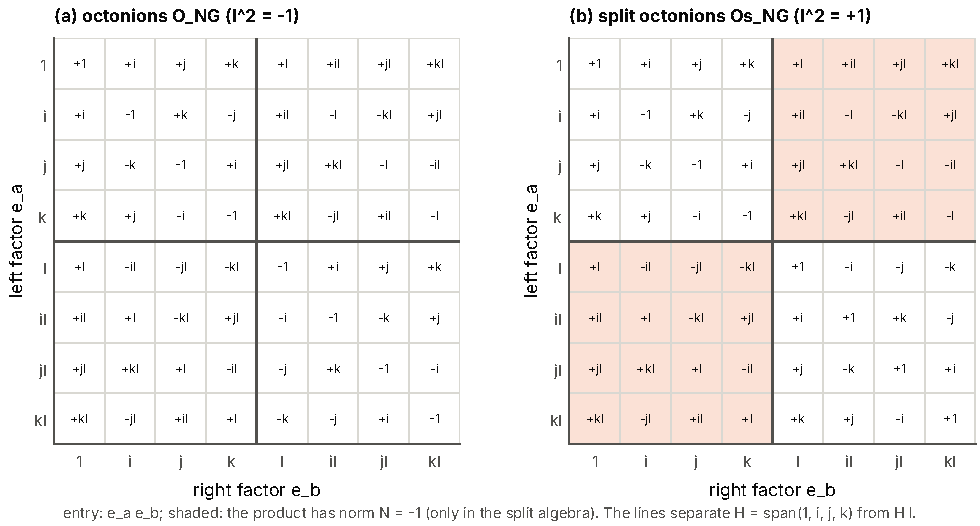
\includegraphics[width=0.92\textwidth]{../figures/fig_ng_tables.pdf}
\caption{Multiplication tables of the octonions (a) and the split octonions (b): the row gives the
left factor, the column the right factor, the entry their product. Shaded: products of norm $-1$
(only in the split algebra). The lines separate the quaternions from their complement. Data:
\texttt{data/ng\_octonion\_tables.csv}.}
\label{fig:tables}
\end{figure*}

The program verifies, in exact integer arithmetic and for both algebras, the following facts
(checks O-1 to O-13 of Appendix~\ref{app:checks}).

\emph{Composition.} $N_{\rm NG}(\mathsf x\mathsf y)=N_{\rm NG}(\mathsf x)N_{\rm NG}(\mathsf y)$. Because both sides
are polynomials of degree four, it suffices to verify the fully polarized identity
$\langle\mathsf x\mathsf y,\mathsf z\mathsf w\rangle_{\rm NG}+\langle\mathsf x\mathsf w,\mathsf z\mathsf y\rangle_{\rm NG}=
2\langle\mathsf x,\mathsf z\rangle_{\rm NG}\langle\mathsf y,\mathsf w\rangle_{\rm NG}$ on all $8^4=4096$ quadruples of
basis elements, which the program does.

\emph{Alternativity and non-associativity.} The associator $(\mathsf x,\mathsf y,\mathsf z)=(\mathsf x\mathsf y)\mathsf z-
\mathsf x(\mathsf y\mathsf z)$ is trilinear, so it is known once it is known on basis elements. It is
totally antisymmetric (the algebras are \emph{alternative}), but it is not zero: it vanishes on
{{GEN:assoc_zero}} of the 512 ordered triples of basis elements and is nonzero on the other
{{GEN:assoc_nonzero}}, which are the triples of three different imaginary units that do not lie in one
quaternionic subalgebra; for example $(\mathsf e_1,\mathsf e_2,\mathsf e_4)=\mathsf e_3\mathsf e_4-\mathsf e_1\mathsf e_6=
\mathsf e_7-(-\mathsf e_7)=2\mathsf e_7$. Alternative algebras obey the Moufang identities
$\mathsf z(\mathsf x(\mathsf z\mathsf y))=((\mathsf z\mathsf x)\mathsf z)\mathsf y$, $\mathsf x(\mathsf z(\mathsf y\mathsf z))=
((\mathsf x\mathsf z)\mathsf y)\mathsf z$ and $(\mathsf z\mathsf x)(\mathsf y\mathsf z)=(\mathsf z(\mathsf x\mathsf y))\mathsf z$; the
program confirms them on 2000 random triples with integer coefficients.

\emph{The commutator algebra is not a Lie algebra.} The commutator $[\mathsf x,\mathsf y]=\mathsf x\mathsf y-
\mathsf y\mathsf x$ of two imaginary elements is imaginary. Its Jacobiator
\begin{equation}
\mathrm{Jac}_{\rm NG}(\mathsf x,\mathsf y,\mathsf z)=[[\mathsf x,\mathsf y],\mathsf z]+[[\mathsf y,\mathsf z],\mathsf x]+[[\mathsf z,\mathsf x],\mathsf y]
\label{eq:jacobiator}
\end{equation}
is, in any algebra, the sum of the six associators of $\mathsf x,\mathsf y,\mathsf z$ taken in all orders
with the signs of the permutations; in an alternative algebra each of them equals $(\mathsf x,\mathsf y,\mathsf z)$
times that sign, so $\mathrm{Jac}_{\rm NG}(\mathsf x,\mathsf y,\mathsf z)=6(\mathsf x,\mathsf y,\mathsf z)$, which the program verifies
on all basis triples. The Jacobiators of the imaginary basis elements span all seven imaginary
directions (rank 7). The imaginary octonions with this commutator form a Malcev
algebra~\cite{Malcev1955} (they satisfy the Malcev identity $\mathrm{Jac}_{\rm NG}(\mathsf x,\mathsf y,[\mathsf x,\mathsf z])=
[\mathrm{Jac}_{\rm NG}(\mathsf x,\mathsf y,\mathsf z),\mathsf x]$, checked), not a Lie algebra.

\emph{Theorem 1 (octonionic charges have no operator representation).} Let $\rho_{\rm NG}$ be a linear
map from the imaginary octonions (or split octonions) to the linear operators on some vector space
with $\rho_{\rm NG}([\mathsf x,\mathsf y])=\rho_{\rm NG}(\mathsf x)\rho_{\rm NG}(\mathsf y)-\rho_{\rm NG}(\mathsf y)
\rho_{\rm NG}(\mathsf x)$. Then $\rho_{\rm NG}=0$.
\emph{Proof.} Products of operators are associative, so the Jacobiator of any three operators
vanishes, and $\rho_{\rm NG}(\mathrm{Jac}_{\rm NG}(\mathsf x,\mathsf y,\mathsf z))=0$. Since the Jacobiators span all imaginary
elements, $\rho_{\rm NG}$ vanishes on all of them. $\square$

Charges that obey the octonionic commutation relations therefore cannot be generators of
symmetries in any quantum theory on a Hilbert space (hypothesis H0): the non-associativity of the
octonions removes them from the reach of the no-go theorems only by removing them from quantum
mechanics. (Octonionic quantum mechanics exists only for the exceptional Jordan algebra of $3\times3$
octonionic Hermitian matrices~\cite{JordanNeumannWigner1934,GunaydinPironRuegg1978}, which has no
tensor products and hence no scattering of several particles.) What survives in quantum mechanics
is the associative envelope: the left multiplications $L_{\rm NG}(\mathsf x)$, $\mathsf y\mapsto\mathsf x\mathsf y$,
are $8\times8$ matrices, and the Lie algebra that the seven $L_{\rm NG}(\mathsf e_1),\dots,
L_{\rm NG}(\mathsf e_7)$ generate under commutators has dimension 28 and is the whole rotation algebra
$\mathfrak{so}(8)$ (octonions) or $\mathfrak{so}(4,4)$ (split octonions) of the norm (check O-12). In the
associative world the octonionic ``charges'' \emph{are} rotation generators of eight dimensions.

\emph{Derivations.} A derivation is a linear map $\mathsf D$ with $\mathsf D(\mathsf x\mathsf y)=(\mathsf D\mathsf x)
\mathsf y+\mathsf x(\mathsf D\mathsf y)$; the derivations generate the automorphisms of the algebra. Solving this
linear condition exactly gives a space of dimension 14 for both algebras, inside the rotations of
the imaginary elements. Its Killing form $B_{\rm NG}(\mathsf D_1,\mathsf D_2)=\mathrm{tr}(\mathrm{ad}\,\mathsf D_1\,
\mathrm{ad}\,\mathsf D_2)$ (with $\mathrm{ad}\,\mathsf D_1$ the matrix of the map $\mathsf D\mapsto[\mathsf D_1,\mathsf D]$ of the derivations into themselves) is negative
definite for $\mathbb O_{\rm NG}$, so its derivations form the compact Lie algebra $\mathfrak g_2$ of the
compact group $\mathrm G_2$, and has {{GEN:split_g2_signature}} for $\mathbb O'_{\rm NG}$, the split real
form of $\mathfrak g_2$ (checks O-10, O-11).

\subsection{The Dirac matrices of the two spacetimes are octonionic}

\emph{$7+1$.} Write a point of the $7+1$ spacetime as the octonion
$\mathsf x=x4\,\mathsf e_0+x1\,\mathsf e_1+x2\,\mathsf e_2+x3\,\mathsf e_3+x0\,\mathsf e_4+x5\,\mathsf e_5+x6\,\mathsf e_6+x7\,\mathsf e_7$:
the time is the real part, the three directions of ordinary space are the imaginary quaternions, and
$x0,x5,x6,x7$ are the complement $\mathbb H_{\rm NG}\mathsf e_4$. Denote by $u_{\rm NG}(A)$ the index of the
unit attached to the coordinate $xA$ ($u_{\rm NG}(4)=0$, $u_{\rm NG}(j)=j$, $u_{\rm NG}(0)=4$,
$u_{\rm NG}(t)=t$). The metric $\eta_{1671}=\mathrm{diag}(-1,-1,-1,-1,+1,-1,-1,-1)$ of the $7+1$ spacetime is
then the real part of the square: $\eta_{1671}(\mathsf x,\mathsf x)=(x4)^2-\sum_{A\ne4}(xA)^2=\mathrm{Re}(\mathsf x^2)$
(check O-14c). The sixteen-dimensional matrices
\begin{align}
\Gamma^4_{71\rm NG}&=\begin{pmatrix}0&\mathsf 1_8\\ \mathsf 1_8&0\end{pmatrix},\nonumber\\
\Gamma^A_{71\rm NG}&=\begin{pmatrix}-L_{\rm NG}(\mathsf e_{u_{\rm NG}(A)})&0\\0&L_{\rm NG}(\mathsf e_{u_{\rm NG}(A)})\end{pmatrix}
\label{eq:gamma71oct}
\end{align}
($A\neq4$; $\mathsf 1_8$ is the unit matrix) satisfy $\Gamma^A_{71\rm NG}\Gamma^C_{71\rm NG}+
\Gamma^C_{71\rm NG}\Gamma^A_{71\rm NG}=2\eta_{1671}^{AC}\mathsf 1_{16}$: for an imaginary unit $\mathsf e$,
alternativity gives $\mathsf e(\mathsf e\mathsf y)=\mathsf e^2\mathsf y=-\mathsf y$, so $L_{\rm NG}(\mathsf e)^2=-\mathsf 1_8$, and
for two different imaginary units $\mathsf e(\mathsf f\mathsf y)+\mathsf f(\mathsf e\mathsf y)=(\mathsf e\mathsf f+\mathsf f\mathsf e)\mathsf y=0$
(check O-14a).

\emph{$4+4$.} Write a point as the split octonion $\mathsf x=\sum_A xA\,\mathsf e_A$. The metric
$\eta_{1644}=\mathrm{diag}(+1,+1,+1,+1,-1,-1,-1,-1)$ is the norm, $\eta_{1644}(\mathsf x,\mathsf x)=N_{\rm NG}(\mathsf x)$
(check O-14d), and the matrices
\begin{equation}
\Gamma^A_{44\rm NG}=\begin{pmatrix}0&L_{\rm NG}(\bar{\mathsf e}_A)\\L_{\rm NG}(\mathsf e_A)&0\end{pmatrix}
\label{eq:gamma44oct}
\end{equation}
satisfy the Clifford relations of $\eta_{1644}$, because $L_{\rm NG}(\bar{\mathsf x})L_{\rm NG}(\mathsf x)=
N_{\rm NG}(\mathsf x)\mathsf 1_8$ in a composition algebra (check O-14b).

\emph{Equivalence with the matrices of the project.} The project's Dirac matrices
$\gamma^A_{1671}$ and $\gamma^A_{1644}$ are built from octonion and split-octonion matrices
$\tau^A_{1671}$ and $\tau^A_{1644}$, $\bar\tau^A_{1644}$ in another basis. Two sets of matrices that
satisfy the same Clifford relations are related by a fixed invertible matrix: with $\gamma^K_{1671}$
the ordered product of the $\gamma^A_{1671}$ over an index set $K$, and $\Gamma^K_{71\rm NG}$ the same
product of the $\Gamma^A_{71\rm NG}$, the matrix
\begin{equation}
\mathcal I_{71\rm NG}=\sum_K\Gamma^K_{71\rm NG}\,\mathsf U_{\rm NG}\,(\gamma^K_{1671})^{-1}
\label{eq:intertwiner}
\end{equation}
(sum over the 256 index sets, $\mathsf U_{\rm NG}$ a fixed matrix with one entry 1 and all others 0) obeys
$\mathcal I_{71\rm NG}\gamma^A_{1671}=\Gamma^A_{71\rm NG}\mathcal I_{71\rm NG}$, because multiplying by
$\Gamma^A_{71\rm NG}$ on the left and by $(\gamma^A_{1671})^{-1}$ on the right only permutes the terms.
The program computes $\mathcal I_{71\rm NG}$ and the corresponding matrix $\mathcal I_{44\rm NG}$ of $4+4$ (the same
sum with $\Gamma^K_{44\rm NG}$ and $\gamma^K_{1644}$) in integers, finds them invertible (rank 16), and
finds the 256 products $\gamma^K_{1671}$ (and $\gamma^K_{1644}$) linearly independent, so that the
representation is irreducible and the intertwiner is unique up to a factor (check O-15; the two
matrices are in \texttt{data/ng\_intertwiner\_1671.csv} and \texttt{\_1644.csv}). Every statement about the
$\Gamma^A_{71\rm NG}$ or the $\Gamma^A_{44\rm NG}$ is therefore a statement about the $\gamma^A_{1671}$ or the
$\gamma^A_{1644}$ of the project.
